\documentclass[a4paper, 10pt, final, garamond]{book}
\usepackage{cours-preambule}
\graphicspath{{./figures/}}
\addto\captionsfrench{\renewcommand{\figurename}{Fig.}}

\makeatletter
\renewcommand{\@chapapp}{Contr\^ole de connaissances}
\makeatother

% \toggletrue{student}
% \toggletrue{corrige}
\renewcommand{\mycol}{black}
% \renewcommand{\mycol}{gray}

\begin{document}
\setcounter{chapter}{0}

\settype{enon}
\settype{solu}

\chapter{Miroirs et lentilles\ifstudent{~(15')}}

\begin{enumerate}[label=\sqenumi, leftmargin=10pt]
	\item[n]{1}%
	Citer le nom des trois propriétés d'un rayon lumineux.
	\smallbreak
	\psw{%
		Propagation rectiligne dans un milieu TLHI, indépendance des rayons
		lumineux, retour inverse dans un milieu TLI.
	}%
	\item[n]{5} %
	Pour un rayon passant d'un milieu d'indice $n_1$ à un milieu d'indice $n_2$, à
	quelle condition peut-on avoir réflexion totale~? Tracer un schéma d'une
	situation de réflexion totale en nommant l'angle d'incidence. Déterminer
	l'angle de réflexion limite.
	\smallbreak
	\noindent
	\begin{isd}[righthand ratio=.3]
		\psw{%
			On peut avoir réflexion totale uniquement si $n_2 < n_1$. \pt{1}
			Soit $i\ind{lim}$ l'angle d'incidence limite de réfraction. On a alors~:
			\begin{equation*}
				i_2 \stm{=} \frac{\pi}{2}
				\Ra
				\sin(i_2) = 1
			\end{equation*}
			Or, $n_2\sin(i_2) = n_1\sin(i\ind{lim})$ \pt{1} (loi de
			\textsc{Snell-Descartes} pour la réfraction). Ainsi,
			\begin{gather*}
				n_2 \underbracket[1pt]{\cancel{\sin(i_2)}}_{=1} = n_1\sin(i\ind{lim})
				\Lra
				\frac{n_2}{n_1} = \sin(i\ind{lim})
				\Ra
				\boxed{i\ind{lim} \stm{=} \arcsin \left( \frac{n_2}{n_1} \right)}
			\end{gather*}
		}%
		\vspace*{-20pt}
		\tcblower
		\vspace{-15pt}
		\begin{center}
			\sswitch{%
				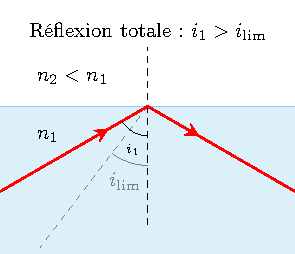
\includegraphics[width=\linewidth, draft=true]{refl_tot-3}
			}{%
				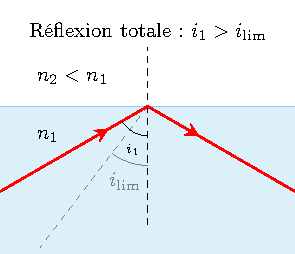
\includegraphics[width=\linewidth]{refl_tot-3}
			}%
			\captionof{figure}{Schéma. \protect \pt{1}}
		\end{center}
	\end{isd}
	\item[n]{6} %
	Démontrer, avec un schéma comportant le tracé de 2 rayons incidents et 2
	rayons émergents, la relation de conjugaison d'un miroir plan. Donner sans
	démonstration son grandissement. Donner, sans schéma, les relations de
	conjugaison des lentilles minces.
	\smallbreak
	\noindent
	\begin{isd}[righthand ratio=.25]
		\vspace{-30pt}
		\psw{%
			\begin{gather*}
				\tan(i) =
				\frac{\obarr{HI}}{\obarr{HA}} \stm{=}
				\frac{\obarr{HI}}{-\obarr{HA'}}
				\Lra
				\boxed{\obarr{HA'} \stm{=} -\obarr{HA}}
				\qav
				\boxed{\gamma = +1} \pt{1}
			\end{gather*}
			et
			\[
				\boxed{ \frac{1}{\OFp} \stm{=} \frac{1}{\OAp} - \frac{1}{\OA}}
				\qou
				\boxed{-f'^2 \stm{=} \obarr{F'A'}\obarr{FA}}
			\]
		}%
		\vspace*{-20pt}
		\tcblower
		\begin{center}
			\sswitch{%
				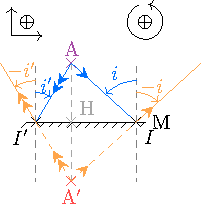
\includegraphics[scale=1, draft=true]{mir_plan-obj_r}
			}{%
				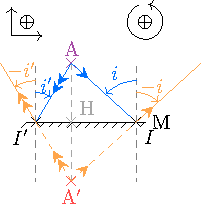
\includegraphics[scale=1]{mir_plan-obj_r}
			}%
			\captionof{figure}{Schéma. \protect \pt{1}}
		\end{center}
		\vspace{-30pt}
	\end{isd}
	\item[n]{8} %
	Construire les images dans les situations suivantes.
	\begin{center}
		\begin{tabular}{cc}
			\sswitch{%
				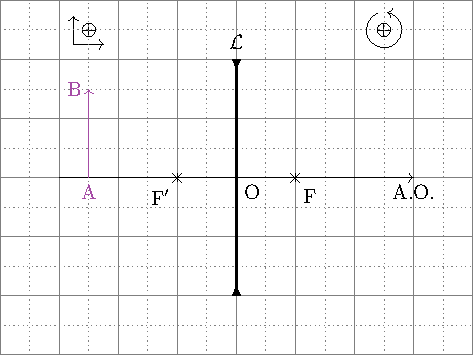
\includegraphics[width=.35\linewidth]{lent_div-constru_simple-plain}
			}{%
				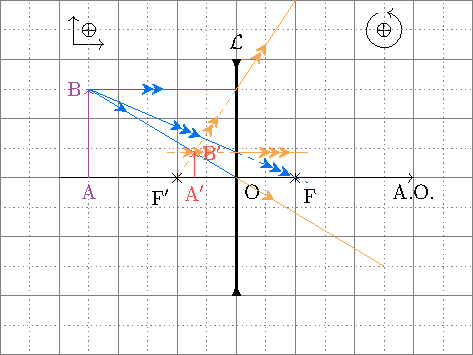
\includegraphics[width=.35\linewidth]{lent_div-constru_simple}
			}%
			 &
			\sswitch{%
				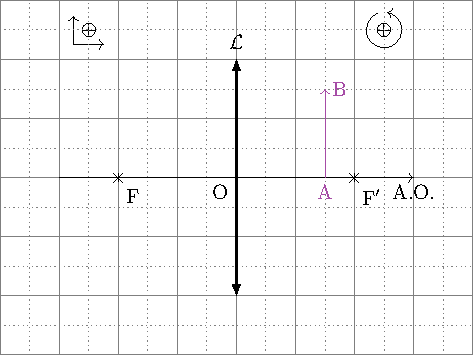
\includegraphics[width=.35\linewidth]{lent_conv-constru_after-plain}
			}{%
				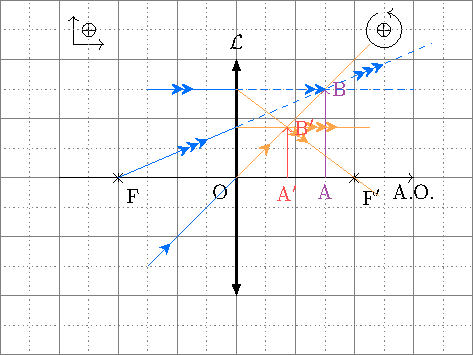
\includegraphics[width=.35\linewidth]{lent_conv-constru_after}
			}%
			\\
			\sswitch{%
				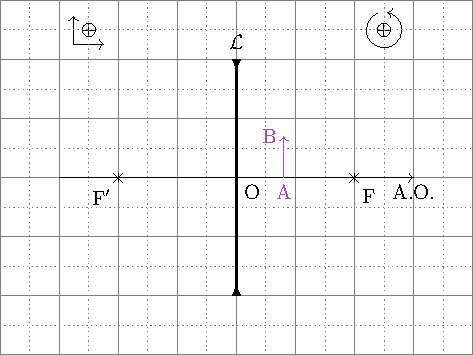
\includegraphics[width=.35\linewidth]{lent_div-constru_after_a-plain}
			}{%
				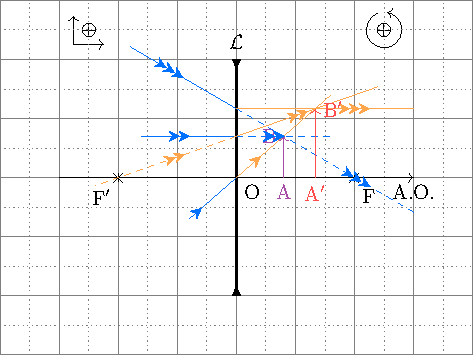
\includegraphics[width=.35\linewidth]{lent_div-constru_after_a}
			}%
			 &
			\sswitch{%
				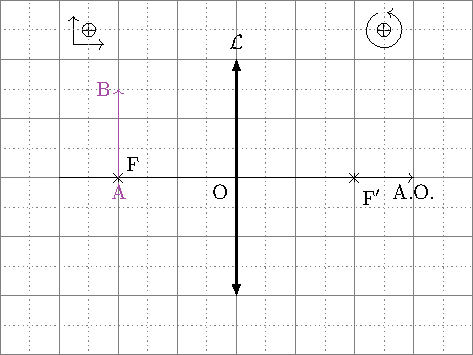
\includegraphics[width=.35\linewidth]{lent_conv-constru_F-plain}
			}{%
				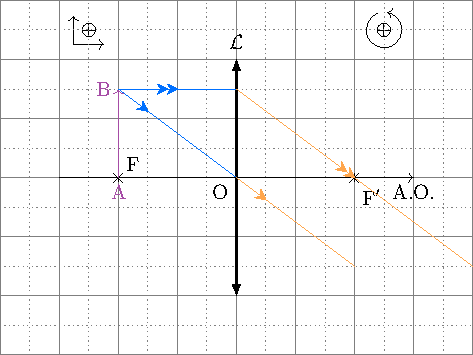
\includegraphics[width=.35\linewidth]{lent_conv-constru_F}
			}%
		\end{tabular}
	\end{center}
\end{enumerate}
\vspace{-30pt}

\ifstudent{
	\begin{tikzpicture}[remember picture, overlay]
		\node[anchor=north west, align=left]
		at ([shift={(1.4cm,0)}]current page.north west)
		{\\[5pt]\Large\bfseries Nom~:\\[10pt]\Large\bfseries Prénom~:};
		\node[anchor=north east, align=right]
		at ([shift={(-1.5cm,-17pt)}]current page.north east)
		{\Large\bfseries Note~:\hspace{1cm}/20};
	\end{tikzpicture}
}

\end{document}
